\chapter{\texttt{FCC}}

\section{Projet FCC}

\subsection{Présentation}

Le FCC (Futur Collisionneur Circulaire) est le projet du CERN pour remplacer 
leur collisionneur actuelle, le LHC (Large Hadronic Collider). 
Dont la fin de l'exploitation est prévu en 2040 \cite{cern:fcc}

Pour le FCC, on prévoit un anneau de 100 km, contre 27 km pour le LEP et le LHC 
(comme montrer Figure~\cite{fcc:img}).
Ce qui devrait nous permettra d'atteindre une énergie de 100 TeV contre 13 TeV
actuellement pour le LHC.

L'objectif est de rechercher d'une nouvelle physique, en mettant au jour de 
déviation avec le modèle standard.


\begin{figure}[h!]
    \centering
    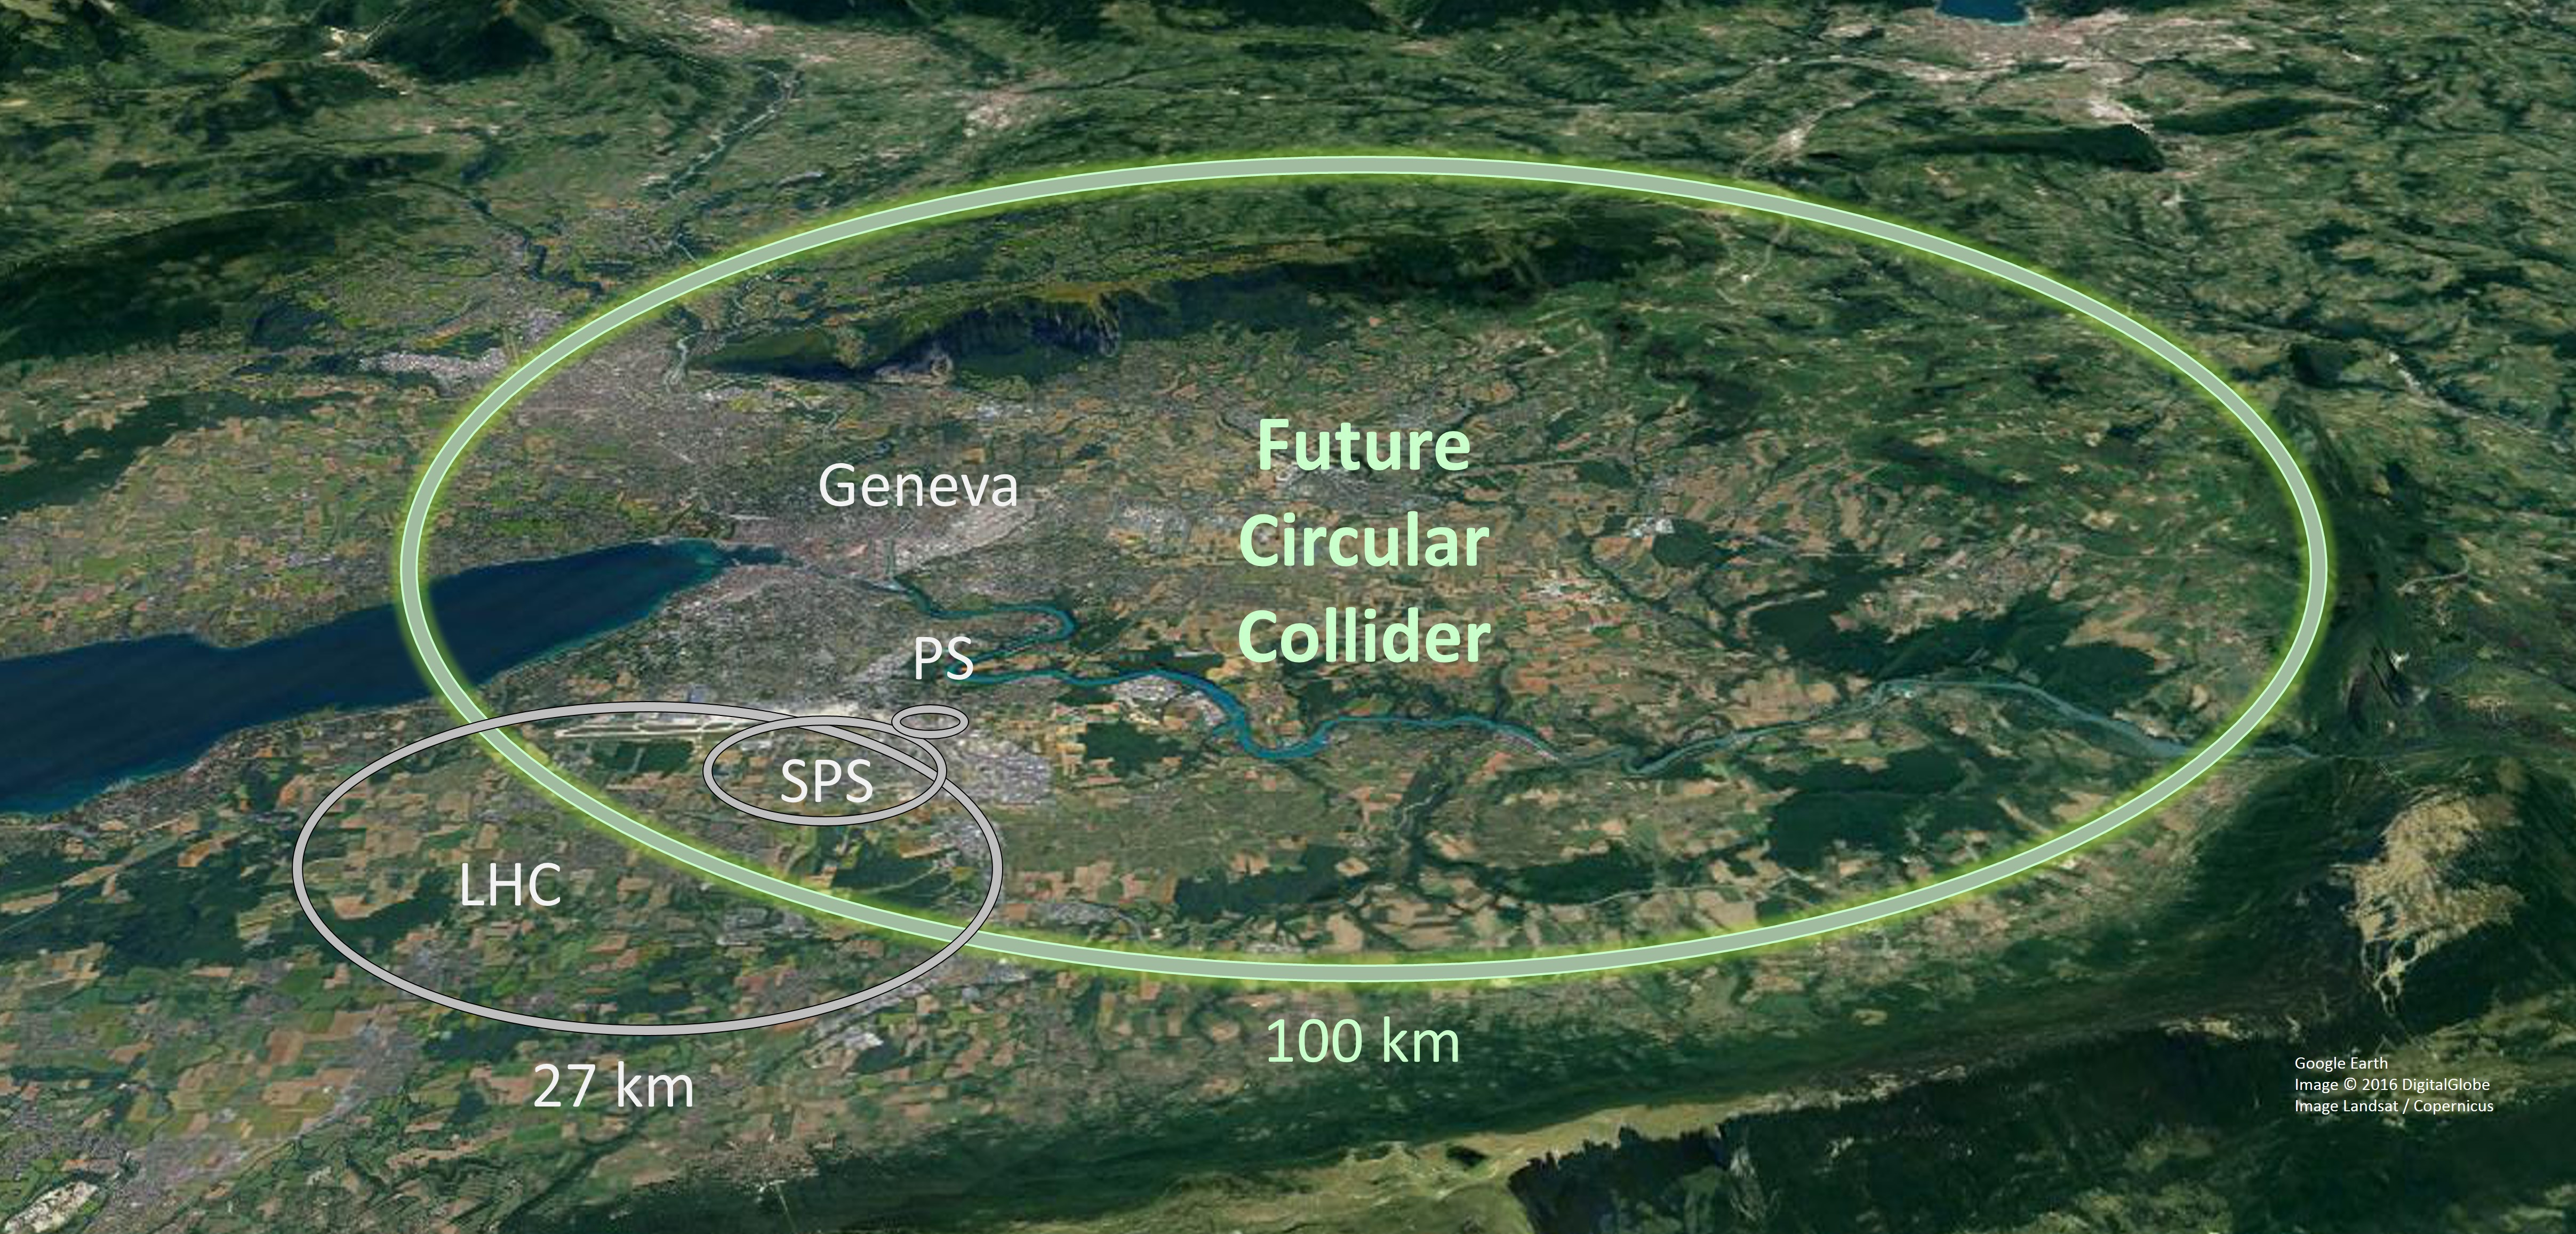
\includegraphics[width=\textwidth]{../img/FCC.jpg}
    \caption{https://cds.cern.ch/images/OPEN-PHO-ACCEL-2019-001-2}
    \label{fcc:img}
\end{figure}

\section{Développement Numérique}

Mon objectif dans ce stage est de transformer les codes développés par Guillaume 
\textsc{Garillot} lors de son post-doctorat pour le projet ILC pour ce projet 
qui n'utilise pas les mêmes suites logiciels.

\texttt{Gaudi}

\texttt{EDM4hep}

\section{Travail de Stage}

\section{Comparaison avec \texttt{iLCSoft}}
